\graphicspath{{img/intro/}}
\phantomsection
\addcontentsline{toc}{chapter}{Introduzione}
\chapter*{Introduzione}

\par Il corso ``Laboratorio di progettazione in alta frequenza'' ha avuto l'obiettivo di introdurre gli studenti alla progettazione di sistemi e circuiti a radiofrequenza, partendo dalle basi teoriche fino ad arrivare alla realizzazione pratica di alcuni sistemi a radiofrequenze (RF). Nel corso delle esercitazioni siamo andati ad affrontare problemi gradualmente pi� complessi per riuscire a realizzare un sistema completo di ricetrasmissione. Partendo dal problema dell'adattamento, fondamentale per questi circuiti, passando alla realizzazione di un \itt{power detector}, circuito ormai presente nella maggior parte dei prodotti commerciali relativi alle comunicazioni mobili, fino alla progettazione vera e propria di un \itt{transceiver} basato su modulazione FSK operante nella banda ISM a 2.4 GHz. Durante queste esperienze abbiamo sfruttato uno dei CAD (\itt{Computer Aided Design}) commerciali pi� conosciuti e utilizzati, cio� Advanced Design System (ADS) della Agilent Technologies \cite{AgBroch}.

\par La popolarit� di questo software, o per meglio dire di questo pacchetto di software, � dovuta principalmente alla sua versatilit�, in quanto supporta la progettazione e lo sviluppo di una vasta gamma di sistemi RF, dai pi� semplici ai pi� complessi, dai moduli a microonde MCM (\itt{MultiChip Modules}) fino agli integrati monolitici (MMIC) utilizzati sia per le telecomunicazioni che per le applicazioni aerospaziali e militari.

\par Al giorno d'oggi infatti la complessit� della progettazione di sistemi wireless � molto elevata a causa dei nuovi standard emergenti come WLAN, UWB, 3GPP, Digital TV, e il WiMAX, mentre il \itt{time to market} richiesto continua a diminuire soprattutto per quanto riguarda le applicazioni nelle comunicazioni ed in ambito aerospaziale e militare. Queste ultime richiedono una completa verifica del sistema, oltre a delle misure efficienti (in termini temporali) e ben documentate. Diventa fondamentale quindi uno strumento CAD in grado di assistere in tutte le fasi della progettazione, dividendo il design dell'intero sistema in una parte RF ed una in banda base, oltre a permettere lo studio delle connessioni fisiche a livello hardware ed una simulazione di tipo elettromagnetico. In questo modo, grazie ad un set completo di tecnologie che coprono sia le simulazioni circuitali nel dominio del tempo e della frequenza che le simulazioni di tipo elettromagnetico, ADS permette ai progettisti una caratterizzazione totale del sistema. L'ambiente di sviluppo, oltre alle simulazioni, permette anche di rappresentare graficamente gli schematici e i \itt{layout}, e include la possibilit� di aggiornare i simulatori, i modelli di riferimento e le librerie di componenti.

\begin{figure}[ht!]
\centering
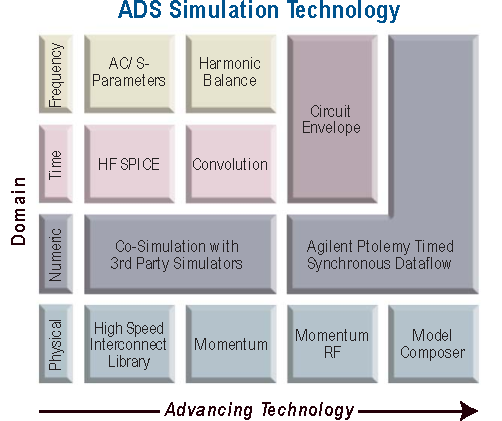
\includegraphics[width=12cm]{ADSSimTecno}
\caption{Simulatori RF che costituiscono l'ambiente ADS.}
\label{fig:ADSSimTecno}
\end{figure}

\par Nella figura \ref{fig:ADSSimTecno} sono rappresentate tutte le simulazioni in alta frequenza che il programma � in grado di effettuare ed i rispettivi domini in cui esse operano; la combinazione di esse permette appunto di caratterizzare e ottimizzare completamente il design del nostro sistema sotto opportune condizioni. In particolare, nel corso delle nostre esercitazioni abbiamo utilizzato solo alcuni di questi simulatori, il cui funzionamento dettagliato � rimandato al seguito quando saranno davvero sfruttate. Di seguito diamo solo alcuni cenni sui simulatori pi� importanti che costituiscono il \itt{design flow} di ADS.

\begin{figure}[ht!]
\centering
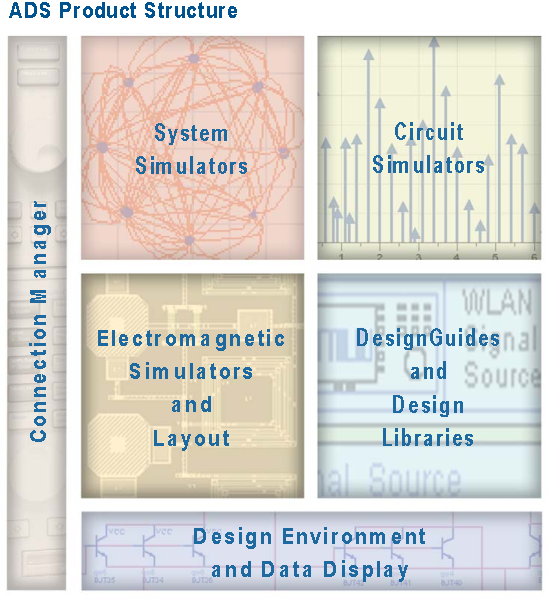
\includegraphics[width=10cm]{ADSProdStruct}
\caption{Interoperabilit� dei simulatori di ADS.}
\label{fig:ADSProdStruct}
\end{figure}

\par Per simulazioni a livello di sistema, l'\itt{Agilent Ptolemy Timed Synchronous Data Flow} \cite{Ptolemy} garantisce l'interoperabilit� tra i vari simulatori concordando i dati ottenuti ai vari livelli circuitali. Ptolemy permette quindi di analizzare le \itt{performances} di sistema ad esempio tramite \itt{bit error rate} e diagrammi delle costellazioni. Il simulatore \itt{Harmonic Balance} � stato invece introdotto per la prima volta dall' Agilent Technologies agli inizi degli anni ottanta ed � diventato il simulatore pi� importante nel dominio della frequenza per ottenere delle analisi rapide di circuiti non lineari, come verr� spiegato meglio in seguito. Oggi � in grado di gestire circuiti integrati ad alta densit� (VLSI) e pu� anche simulare divisori di frequenza digitali, sfruttando le capacit� del simulatore \itt{Transient} col \itt{Transient Assisted Harmonic Balance}. Il simulatore \itt{Circuit Envelope} invece � un'innovazione brevettata da Agilent che permette un'analisi accurata di un segnale modulato direttamente nel dominio della frequenza. Il simulatore \itt{RF System} realizza un'analisi di sistema ad alto livello, fornendo per ogni componente tutta una serie di parametri fondamentali quali cifra di rumore, IP3, 1 dBC, ecc. 
\par Un'accurata implementazione a livello fisico del circuito � di vitale importanza per predire le performance a livello hardware; per questo ADS include anche un ambiente di sviluppo fisico opportunamente congegnato per design di layout alle alte frequenze. Esso offre un elevato numero di capacit�, come la sincronizzazione del progetto con lo schematico; l'impiego di un motore per le interconnessioni fisiche ({real time}, che gira senza bisogno di dover lanciare nessuna utility secondaria) con \itt{Design Rule Checker} (DRC); la disponibilit� di simulatori elettromagnetici per circuiti planari come il \itt{Momentum} (2.5 D) completamente integrato con l'ambiente del layout. In questo modo aumenta per i progettisti la possibilit� di rilevare errori prima della produzione.
\par Un altro punto a favore della flessibilit� di questo software risulta essere la compatibilit� con molti altri design flow commerciali, ad esempio quelli basati su Cadence e Mentor, per citare alcuni dei pi� noti; in questo modo aumenta molto l'integrazione di quei prodotti che usano standard commerciali. 
\par Infine per quanto riguarda i problemi ad alta frequenza (riflessioni, {crosstalk}, ritardi di propagazione, integrit� del segnale, temporizzazioni, ecc.) ormai all'ordine del giorno nei circuiti che sfruttano clock ad altissima velocit�, ADS � in grado di modellarli e analizzarli con accuratezza grazie a librerie e ad opportuni strumenti di simulazione. In questo modo � possibile diminuire i problemi di interconnessioni ad alta frequenza prima della fabbricazione, riducendo quindi i costi e velocizzando il time to market.


%\par Il progetto di dispositivi di ricetrasmissione alle frequenze delle microonde richiede l'impiego di modelli accurati, che rispecchino il comportamento elettromagnetico dei componenti circuitali utilizzati e delle loro interconnessioni, le cui dimensioni diventano confrontabili con la lunghezza d'onda dei segnali informativi trattati.
%\par In alta frequenza, i componenti circuitali fisici presentano componenti parassiti non pi� trascurabili, e le loro impedenze possono fortemente discostarsi dal valore nominale atteso. Inoltre, i collegamenti tra i componenti diventano vere e proprie linee di trasmissione, per le quali � necessario conoscere l'impedenza caratteristica ai fini di un corretto convogliamento del segnale mediante gli opportuni adattamenti di impedenza alle estremit�.
%\par Vi � la necessit� di adattare, localmente, l'impedenza di uscita di un blocco a monte all'impedenza d'ingresso del blocco immediatamente a valle, in modo di massimizzare il trasferimento di potenza e minimizzare il coefficiente di riflessione. Qualsiasi perdita di segnale necessita di meccanismi di rigenerazione, operazioni che introducono rumore particolarmente degradante nella catena di ricezione.
%
%
%\par Le tecniche odierne di progettazione di circuiti in alta frequenza richiedono l'impiego di strumenti CAD\footnote{Computer Aided Design.} sofisticati che permettano di simulare il comportamento di tali circuiti.
%
%\DeclareFixedFootnote{\rep}{Text to repeat}
%
%
%
